\subsubsection{Command line utility}\label{sec:command-line-utility}

Not everyone who could benefit
from my application
needs to have a good understanding
of Go development.
That is why I also prepared
a command line utility
that is compatible with the most popular shells:
Unix-like shells,
and Powershell.

Its feature set is very similar
to the one mentioned in the previous section,
but it also includes configuration files support,
and notification templates for convenience.
This in turn enables its users
to set up the producer for multiple Apps
on one system.
It is only necessary to provide
separate configuration files
and, optionally, separate notification templates.
An example of such setup is presented
in figures~\ref{fig:notipie-one-notification}
and~\ref{fig:notipie-two-notifications}.

\paragraph*{Configuration and notification templates}\label{sec:configuration-and-notification-templates}

This version of a producer can be configured
either through the command line arguments
or the configuration files,
but the command line arguments
always take precedence.
The configuration files themselves
can be stored in \ac{JSON} or \ac{YAML} format.
I chose those two,
because they are very popular
for this use case.
These formats can also be used
for specifying a notification template.

The configuration consists of
the address and port of the backend,
which are set by user.
Also, when the producer sends its first notification
and gets back the App \ac{ID},
the producer appends it to the configuration file,
so that it is present in every consecutive push.

The notification template can be any
subset of an App notification model
defined in section~\ref{sec:protocol}.
Everything specified in this template
can be overwritten with \ac{CLI} arguments.
The only requirement for a valid request
is to have an App name and title set.
The timestamp is set automatically for us.

\paragraph*{Usage}\label{sec:producer-usage}

As described in the previous section,
the producer allows different configurations
for one \ac{CLI} program,
enabling user to set up many different Apps
on the same computer.
Figures~\ref{fig:notipie-one-notification}
and~\ref{fig:notipie-two-notifications}
show the producer sending the notifications
to the Notipie \ac{UI}.
The producer is executed
with different configurations
and notification templates.
The configurations only differ
in the randomly-generated App \ac{ID}.

\begin{figure}[!p]
  \centering
  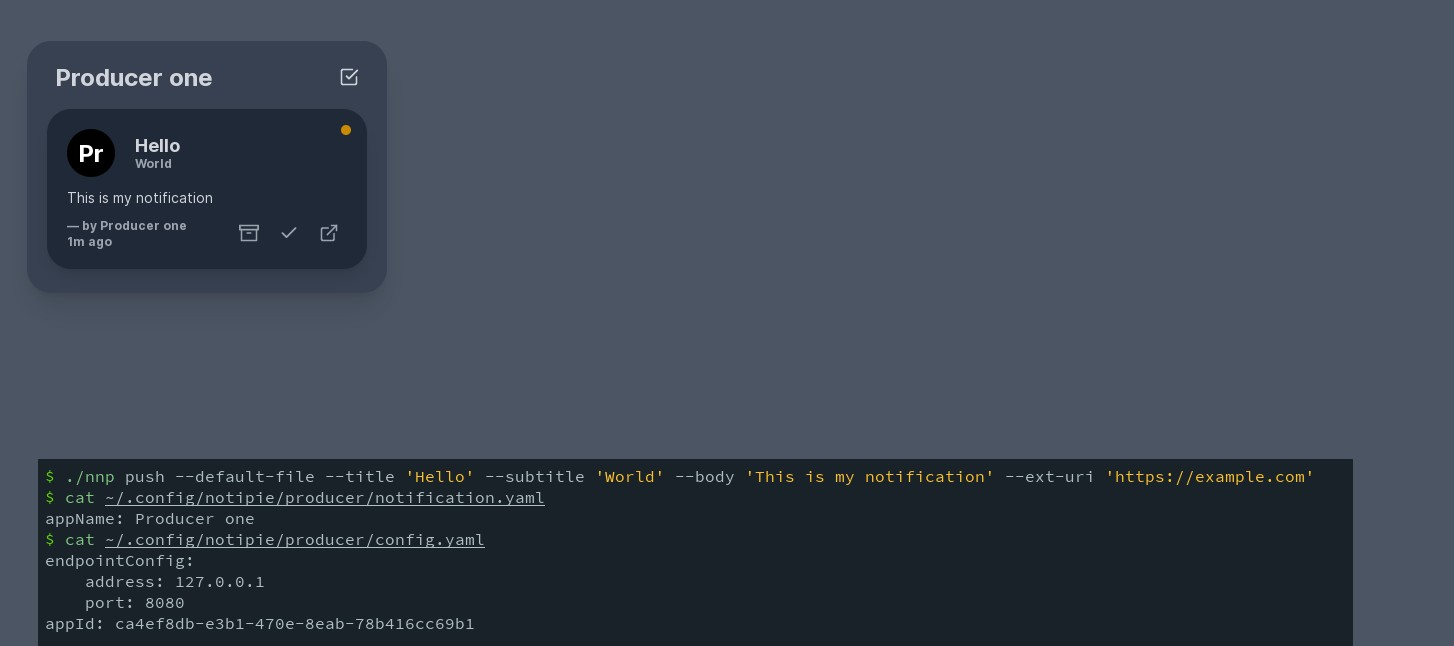
\includegraphics[width=\linewidth,keepaspectratio]{img/notipie_one_notification.jpg}
  \caption{First producer pushing a notification to the UI}
  \label{fig:notipie-one-notification}
\end{figure}

\begin{figure}[!p]
  \centering
  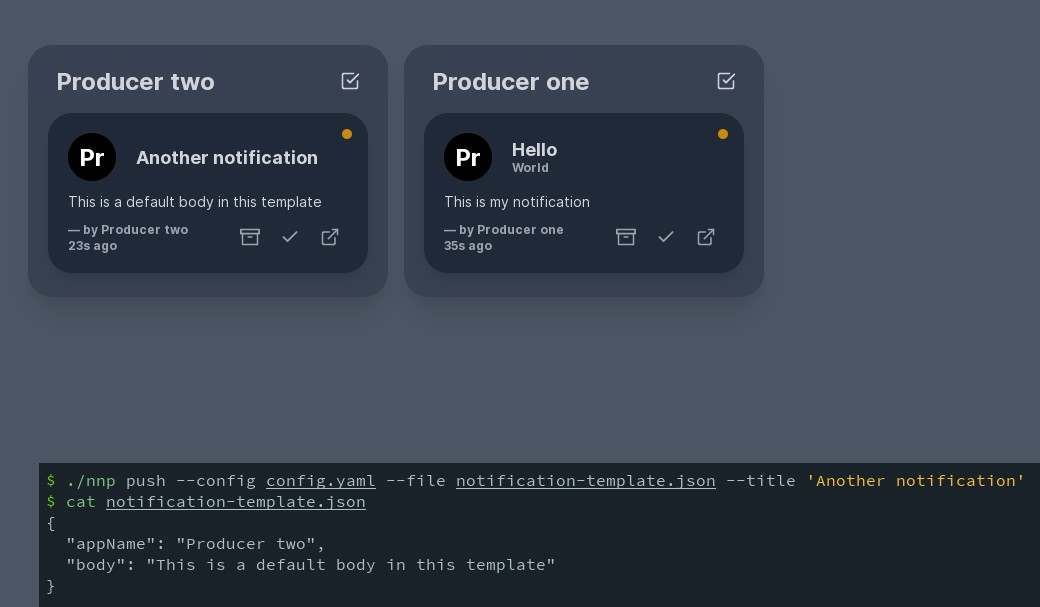
\includegraphics[width=\linewidth,keepaspectratio]{img/notipie_two_notifications.jpg}
  \caption{Second producer pushing a notification to the UI}
  \label{fig:notipie-two-notifications}
\end{figure}
